\documentclass[11pt]{beamer}
\usetheme{Warsaw}
\usepackage[utf8]{inputenc}
\usepackage[english]{babel}
\usepackage{amsmath}
\usepackage{amsfonts}
\usepackage{amssymb}

%expectations
\newcommand{\expect}{\mathbb{E}}

\AtBeginSection[]{
  \begin{frame}
  \vfill
  \centering
  \begin{beamercolorbox}[sep=8pt,center,shadow=true,rounded=true]{title}
    \usebeamerfont{title}\insertsectionhead\par%
  \end{beamercolorbox}
  \vfill
  \end{frame}
}


\begin{document}
%%%%%%%%%%%%%%%%%%%%%%%%%%%%%%%%%%%%%%%%%%%%%%%%%%%%%%%%
\begin{frame}
  \frametitle{}
  \begin{center}
    \textbf{\large MATH 4281 Risk Theory--Ruin and Credibility}\\
    \vspace{1cm}
    {\large  Module 3: Credibility Theory (cont.)} \\
    \vspace{1cm}
    {\large  March 23th, 2021}
    \end{center}
    \vspace{1cm}
\end{frame}
%%%%%%%%%%%%%%%%%%%%%%%%%%%%%%%%%%%%%%%%%%%%%%%%%%%%%%%%
\begin{frame}
\tableofcontents
\end{frame}
%%%%%%%%%%%%%%%%%%%%%%%%%%%%%%%%%%%%%%%%%%%%%%%%%%%%%%%%
\section{A General Model}
\begin{frame}{A useful result}

For which pairs $f_{X|\Theta}(x|\theta)$ and $\pi(\theta)$ is $P^{Bayes}=\widetilde{\mu(\Theta)}$ linear? Equivalently, when is $\widetilde{\mu(\Theta)}$ of the form
$$\widetilde{\mu(\Theta)}=z \bar{X} + (1-z)m\;?$$
\begin{itemize}
\item It is the case for about half a dozen famous examples.
\item Jewell (1974) unified these examples
\item Gerber (1995) proposed an alternative formulation
\end{itemize}
\end{frame}

\begin{frame}{A general model}
Suppose
\begin{itemize}
\item $$f_{X|\Theta}(x|\theta)=\frac{a(x)\cdot b(\theta)^x}{c(\theta)},\quad x\in A$$
where
$$c(\theta)=\int_A a(x)\cdot b(\theta)^x \text{d}x,$$ and
\item
$$\pi(\theta)=\frac{c(\theta)^{-m_0}\cdot b(\theta)^{x_0}\cdot b'(\theta)}{d(m_0,x_0)},$$
where
$$d(m_0,x_0)=\int c(\theta)^{-m_0}\cdot b(\theta)^{x_0}\cdot b'(\theta) \text{d}\theta.$$
\end{itemize}

\end{frame}
%%%%%%%%%%%%%%%%%%%%%%%%%%%%%%%%%%%%%%%%%%%%%%%%%%%%%%%%
\begin{frame}{A general model}

Then \begin{itemize}
\item
$\pi_\mathbf{x}(\theta)$ is in the same family of $\pi(\theta)$, with the following updated parameter values (for $m_0$ and $x_0$):
$$m_0+T \quad\text{and}\quad x_0+\sum_{j=1}^T X_{j}$$
\item and finally,
$$P^{Bayes}=\widetilde{\mu(\Theta)}=E[\Theta|X]=\frac{x_0+S+1}{m_0+T}
=z\bar{X}+(1-z)m$$
with
$$z=\frac{T}{m_0+T}.$$
\end{itemize}

\end{frame}
%%%%%%%%%%%%%%%%%%%%%%%%%%%%%%%%%%%%%%%%%%%%%%%%%%%%%%%%
\section{B\"uhlmann model}
\begin{frame}{Hans B{\"u}hlmann-Curriculum Vitae}

\begin{columns}
\column{0.35\textwidth}
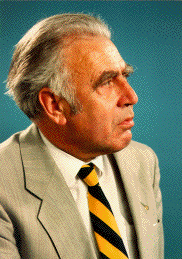
\includegraphics[scale=0.6]{Buehlmannp.png}

\column{0.65\textwidth}
\begin{itemize}
\item PhD ETHZ, 1959
\item Swiss Re, 1958-1961 \& 1963-1966
\item Berkeley, 1961-1963
\item ETHZ, full professor since 1966, Emeritus since 1997, President 1987-1990
\item 5 times \emph{doctor honoris causa}
\item honorary president of ASA and ASTIN
%\item 25 PhD students (of whom Hans U. Gerber \& André Dubey)
\item the father of modern credibility

\item Still alive (91 years old!) and coauthored a book in 2016!
\end{itemize}

\end{columns}

\end{frame}
%%%%%%%%%%%%%%%%%%%%%%%%%%%%%%%%%%%%%%%%%%%%%%%%%%%%%%%%
\begin{frame}{Idea: BLUE vs MVUE}

Consider the following. Going back to the Frequentist world:

\begin{itemize}

\item Given a sample $\lbrace x_1, x_2,..,x_n \rbrace$ drawn from a uniform distribution $X \sim U[0,\theta]$ is $2\bar{x}$ the "best" or "efficient" (minimum variance, unbiased?) statistic for $\theta$?

\vfill

\item The MLE is $\max(x_1, ..., x_n)$ and adjustiing for bias we get $\tilde{\theta} = \frac{n+1}{2n}\max(x_1, ..., x_n)$.

\vfill

\item The MLE is asymptotically efficient and adjusting for bias we \textit{can}\footnote{it's sufficient + Lehmann–Scheffé theorem} show $\tilde{\theta}$ is the MVUE.

\vfill

\item[Q] Wither $\bar{x}$? What special properties does it have in general? 

\item[A] It is BLUE! 

\end{itemize}


\end{frame}
%%%%%%%%%%%%%%%%%%%%%%%%%%%%%%%%%%%%%%%%%%%%%%%%%%%%%%%%
\begin{frame}{Here's the story....
About a little guy that lives in a blue world
...And all day and all night and everything he sees is just blue...}

\begin{itemize}

\item BLUE = Best Linear Unbiased Estimator!

\vfill

\item Sample mean (and OLS in general) guaranteed by theorems like Guass-Markov etc...

\vfill

\item What this means is that for any other linear stat $\ell$:

$$ E[ (\mu(\theta) - \bar{x})^2 ] \leq E[ (\mu(\theta) -  \ell )^2 ] $$


\end{itemize}

\end{frame}
%%%%%%%%%%%%%%%%%%%%%%%%%%%%%%%%%%%%%%%%%%%%%%%%%%%%%%%%
\begin{frame}{Back to the B\"uhlmann model}

Bayes premium is the best possible estimator of all. BUT:

\vfill
\begin{itemize}
\item It does not fulfill the requirement of simplicity (closed analytical results are scarce $\longrightarrow$ tedious numerical procedures)

\vfill

\item One has to specify the conditional and a prior distributions.

\vfill

\item May not have nice form of the kind $z\bar{X}+(1-z)m$.
\end{itemize}


\end{frame}
%%%%%%%%%%%%%%%%%%%%%%%%%%%%%%%%%%%%%%%%%%%%%%%%%%%%%%%%
\begin{frame}{Idea: we restrict to linear estimators}

\begin{itemize}

\item Idea of B\"uhlmann: \\

\begin{center}
``\emph{\alert{restrict}} the class of allowable estimator functions to those which are \alert{\emph{linear}} in the observations $\mathbf{X}$'' 
\end{center}

\vfill

\item We are looking for the \alert{\emph{best estimator}} (in the Bayesian sense) in the class of all \emph{linear estimator functions}. 

\vfill

\item The following estimators are then \alert{linear Bayes estimators}.

\end{itemize}

\end{frame}
%%%%%%%%%%%%%%%%%%%%%%%%%%%%%%%%%%%%%%%%%%%%%%%%%%%%%%%%
\begin{frame}{B\"uhlmann model-Assumptions}

\begin{itemize}
\item 1 insured
\item $\Theta$ risk parameter (random variable)
\item $\Pi(\theta)=\Pr [\Theta\le \theta]$, structural function
\item $X_1,X_2,\ldots,X_T | \Theta$ conditionally iid (given $\Theta$)
\item $\mathbf{x}=(x_1,x_2,\ldots,x_T)'$ observations
\item $\mu(\theta)=E[X_1|\Theta=\theta]$ and $\sigma^2(\theta)=Var(X_1|\Theta=\theta)$
\end{itemize}

\end{frame}
%%%%%%%%%%%%%%%%%%%%%%%%%%%%%%%%%%%%%%%%%%%%%%%%%%%%%%%%
\begin{frame}{B\"uhlmann model-Formulas}

We want to find the best estimator that is linear in the observations:

$$P_{T+1}^{cred}=\sum_{j=1}^T \hat{a}_j X_j + \hat{a}_0$$

such that

$$ E[(\mu(\Theta)-\sum_{j=1}^T \hat{a}_j X_j -\hat{a_0})^2]=\min_{a_0,a_1,\cdots,a_T\in \mathbb{R}}E[(\mu(\Theta)-\sum_{j=1}^T {a}_j X_j -{a_0})^2] $$


\end{frame}
%%%%%%%%%%%%%%%%%%%%%%%%%%%%%%%%%%%%%%%%%%%%%%%%%%%%%%%%
\begin{frame}{B\"uhlmann model-Formulas}

As the distribution of $X_1,\cdots,X_T$ is invariant under permutations of $X_j$, the estimator has the form

$$P_{T+1}^{cred}=z \bar{X} + b,$$

\vspace{0.5 cm}

where $z$ and $b$ are the solution of the minimizing problem

\vspace{0.5 cm}

$$ E[(\mu(\Theta)- z \bar{X} -b)^2]=\min_{a_1,a_0\in \mathbb{R}}E[(\mu(\Theta)-a_1\bar{X} -{a_0})^2] $$ 

\end{frame}
%%%%%%%%%%%%%%%%%%%%%%%%%%%%%%%%%%%%%%%%%%%%%%%%%%%%%%%%
\begin{frame}{B\"uhlmann model-Formulas}

\begin{itemize}
\item
Taking partial derivatives with respect to $a_0$, and $a_1$ respectively:

$$ E[-2(\mu(\Theta)- a_1 \bar{X} -{a_0})]=0 \text{  \&  } E[-2\bar{X}(\mu(\Theta)-a_1\bar{X} -{a_0})]=0$$

\item Solving\footnote{requires a great deal of manipulation etc...not important (pg. 416 of Loss models if you are curious)} the  equations, we get
$$a_1=\frac{Var(\mu(\Theta))}{\frac{E[\sigma^2(\Theta)]}{T}+Var(\mu(\Theta))} \text{  \&  } a_0=(1-a_1)E[\mu(\Theta)].$$

\item Can see $a_1 = z$ (the B\"uhlmann credibility factor) $a_0 = (1-z)m$ as we expected.

\end{itemize}

\end{frame}
%%%%%%%%%%%%%%%%%%%%%%%%%%%%%%%%%%%%%%%%%%%%%%%%%%%%%%%%
\begin{frame}{The credibility premium}

\begin{itemize}
\item The \textbf{credibility premium (credibility estimator)} is then:
    \begin{equation}P_{T+1}^{cred}=z\bar{X} + (1-z)m\end{equation}
    where $$z=\frac{T}{T+K}, \;\;\;K=\frac{E[\sigma^2(\Theta)]}{Var(\mu(\Theta))}$$
and
 $m=E[\mu(\Theta)].$

\item $P^{cred}$ is a weighted mean of $P^{coll}=m$ and the individual observed average $\bar{X}$

\item $K=\frac{E[\sigma^2(\Theta)]}{Var(\mu(\Theta))}$ is called the \textbf{credibility coefficient}
  
\item When the Bayes estimator is linear in the observations, the Bayes estimator is equal to the credibility estimator. We refer to such cases as \textbf{exact credibility}.

\end{itemize}

\end{frame}
%%%%%%%%%%%%%%%%%%%%%%%%%%%%%%%%%%%%%%%%%%%%%%%%%%%%%%%%
\begin{frame}{Example}
\vspace{- 3 cm}
The amount of a claim has the exponential distribution with mean $\frac1{\Theta}$. Among the class of insureds and potential insureds, the parameter $\Theta$ varies according to the gamma distribution  with $\alpha$ and scale parameter $\frac1\beta$.  Suppose that a person had claims of $X_1$, $X_2$, $\cdots$, and $X_n$. Determine the credibility premium of the $n+1$th claim.\\


\end{frame}
%%%%%%%%%%%%%%%%%%%%%%%%%%%%%%%%%%%%%%%%%%%%%%%%%%%%%%%%
\begin{frame}

\end{frame}
%%%%%%%%%%%%%%%%%%%%%%%%%%%%%%%%%%%%%%%%%%%%%%%%%%%%%%%%
\begin{frame}

\end{frame}
%%%%%%%%%%%%%%%%%%%%%%%%%%%%%%%%%%%%%%%%%%%%%%%%%%%%%%%%
\begin{frame}{Quadratic losses}

\alert{$m$}: best estimator based on the a priori knowledge alone. Quadratic loss:
$$E[(m-\mu(\Theta))^2]=Var(\mu(\Theta))=a.$$

\alert{$\bar{X}$}: best linear and individually (conditionally) unbiased (given $\Theta$) estimator, based on the observation vector $\mathbf{X}$. Quadratic loss:
$$E[(\bar{X}-\mu(\Theta))^2]=E[\sigma^2(\Theta)/T]=s^2/T.$$

\alert{$P^{cred}$}: weighted mean of $\bar{X}$ and $m$, where weights are \emph{proportional to their inverse quadratic loss (precision)}

$$ z = \frac{T/s^2}{T/s^2+1/a} \text{  \&  } (1-z)=\frac{1/a}{T/s^2+1/a} $$



\end{frame}
%%%%%%%%%%%%%%%%%%%%%%%%%%%%%%%%%%%%%%%%%%%%%%%%%%%%%%%%
\begin{frame}[t]{Study of $K$}

$$K=\frac{E[\sigma^2(\Theta)]}{Var(\mu(\Theta))} \text{  \&  } z=\frac{T}{T+K} $$

\vfill

The credibility factor $z$ increases as
\vfill
\begin{itemize}
\item the number of observations $T$ increases
\vfill
\item the heterogeneity of the portfolio increases.
\vfill
\item the within risk variability decreases.
\end{itemize}


\end{frame}
%%%%%%%%%%%%%%%%%%%%%%%%%%%%%%%%%%%%%%%%%%%%%%%%%%%%%%%%
\section{Nonparametric estimation}
\begin{frame}{Parametric  and  Nonparametric estimation}

There are three ways of estimating the parameters $m$, $s^2$ and $a$:
\begin{itemize}
\item \alert{Pure Bayesian procedure}: intuitively set using the a priori knowledge of an experienced actuary or underwriter
\item \alert{Parametric estimation}: the distributions $f_{X|\Theta}(x|\theta)$ and $\pi(\theta)$ are known and the parameters are calculated from these distributions.
\item \alert{Nonparametric estimation}: data from a collective of similar risks exist, and values for the parameters are inferred from it. This is an empirical Bayes approach.
\end{itemize}
The parametric estimation is straightforward and follows from the definition of the parameters.

\end{frame}
%%%%%%%%%%%%%%%%%%%%%%%%%%%%%%%%%%%%%%%%%%%%%%%%%%%%%%%%
\begin{frame}{ Nonparametric estimation}

\begin{itemize}
\item $X_{jt}$: claims size of policy $j$ during year $t$.
\item Available data, $1\le j\le J$, $1\le t \le T$:
\begin{tabular}{l|ccccc|cc}
\multicolumn{1}{r}{year $t$} & 1 & 2 & 3 & $\cdots$ & $T$ & Risk & Mean \\ \hline
policy $j=1$ & $X_{11}$ & $X_{12}$ & $X_{13}$ & $\cdots$ & $X_{1T}$ & $\theta_1$ & $\bar{X}_{1\Sigma}$ \\
policy $j=2$ & $X_{21}$ & $X_{22}$ & $X_{23}$ & $\cdots$ & $X_{2T}$ & $\theta_2$ & $\bar{X}_{2\Sigma}$ \\
policy $j=3$ & $X_{31}$ & $X_{32}$ & $X_{33}$ & $\cdots$ & $X_{3T}$ & $\theta_3$ & $\bar{X}_{3\Sigma}$ \\
\multicolumn{1}{c|}{\vdots} & $\vdots$ & $\vdots$ & $\vdots$ & $\ddots$ & $\vdots$ & $\vdots$ & $\vdots$ \\
policy $j=J$ & $X_{J1}$ & $X_{J2}$ & $X_{J3}$ & $\cdots$ & $X_{JT}$ & $\theta_J$ & $\bar{X}_{J\Sigma}$
\end{tabular}
%\item $\Theta_1, \Theta_2,\ldots,\Theta_m$ are iid
\item $X_{11},X_{12},\ldots,X_{JT}$ are $iid$ conditional on $\Theta$.
\item $\mu(\theta_j)=E[X_{jt}|\Theta=\theta_j]$
\item $\sigma^2(\theta_j)=Var(X_{jt}|\Theta=\theta_j)$
\end{itemize}
\begin{columns}
\column{0.8\textwidth}
\begin{equation}\alert{P^{cred}_{j,T+1}=z \bar{X}_{j\Sigma} + (1-z)m,\;\;\;i=1,\ldots,J}\end{equation}
\end{columns}

\end{frame}
%%%%%%%%%%%%%%%%%%%%%%%%%%%%%%%%%%%%%%%%%%%%%%%%%%%%%%%%
\begin{frame}{Nonparametric estimation (unbiaised estimators)}

Estimation of $E[\mu(\Theta)]=m$:
\begin{equation}\bar{X}_{\Sigma\Sigma}=\frac{1}{J}\sum_{j=1}^J \bar{X}_{j\Sigma}=\frac{\sum_{j=1}^J\sum_{t=1}^T X_{jt}}{JT}\end{equation}
Estimation of $E[\sigma^2(\Theta)]=s^2$:
\begin{equation}\hat{s}^2=\frac{1}{J}\sum_{j=1}^J\hat{s}_j^2=\frac{1}{J}\sum_{j=1}^J \sum_{t=1}^T \frac{(X_{jt}-\bar{X}_{j\Sigma})^2}{T-1}\end{equation}

\end{frame}
%%%%%%%%%%%%%%%%%%%%%%%%%%%%%%%%%%%%%%%%%%%%%%%%%%%%%%%%
\begin{frame}{Nonparametric estimation (unbiaised estimators)}
Estimation of $Var(\mu(\Theta))=a$:

(B{\"u}hlmann's estimator)
\begin{equation}\hat{a}_B=Max\left\{\frac{\sum_{j=1}^J(\bar{X}_{j\Sigma}-\bar{X}_{\Sigma\Sigma})^2}{J-1}-\frac{1}{T}\hat{s}^2\;;\;0\right\}\end{equation}

(CAS's estimator)
\begin{equation}\hat{a}_{CAS}=Max\left\{\frac{\sum_{j=1}^J\sum_{t=1}^T(X_{jt}-\bar{X}_{\Sigma\Sigma})^2}{JT-1}-\hat{s}^2\;;\;0\right\}\end{equation}


\begin{itemize}
\item If $\hat{a}=0$ then $z=0$, which makes sense

(all risks have the same parameter)
\end{itemize}

\end{frame}
%%%%%%%%%%%%%%%%%%%%%%%%%%%%%%%%%%%%%%%%%%%%%%%%%%%%%%%%
\begin{frame}{Example 1}
An insurance company sells automobile insurance and has mainly two types of policy: $A$ and $B$. The aggregate claim amounts (in millions of dollars) for the last three years are summarized below:
\begin{center}
\begin{tabular}{ccccc}
\hline Policy Type &  & Year 1 & Year 2 & Year 3 \\ \hline\hline
$A$ &  & 5 & 8 & 11 \\
$B$ &  & 11 & 13 & 12 \\ \hline
\end{tabular}
\end{center}
Estimate the B\"uhlmann's credibility factor and use this to determine the next year's credibility premium for each of the policy type.
\end{frame}

\end{frame}
%%%%%%%%%%%%%%%%%%%%%%%%%%%%%%%%%%%%%%%%%%%%%%%%%%%%%%%%
\begin{frame}

\end{frame}
%%%%%%%%%%%%%%%%%%%%%%%%%%%%%%%%%%%%%%%%%%%%%%%%%%%%%%%%
\begin{frame}

\end{frame}
%%%%%%%%%%%%%%%%%%%%%%%%%%%%%%%%%%%%%%%%%%%%%%%%%%%%%%%%
\end{document}